\documentclass[a4paper,12pt]{article}
\usepackage[english]{babel}
\usepackage[utf8]{inputenc}
\usepackage[T1]{fontenc}
\usepackage{indentfirst}
\usepackage[top=2.5cm, bottom=2.5cm, left=2.5cm, right=2.5cm]{geometry}
\usepackage{amsmath}
\usepackage{hyperref}
\usepackage{graphicx}

\graphicspath{ {./img/} }
\title{ML Nanodegree Capstone Project\\Investment and Trading application}
\author{Maciej Nalepa}
\date{2020 January}
\begin{document}
\maketitle

\part{Definition}
\section*{Project Overview}
Knowing the future of a market stock price is a very valuable information about risk of investment and is commonly pursued because of potentially infinite profits.

Currency ratio and stock markets forecasting based on technical analysis can be easily implemented in a script thanks to a timeseries prediction nature of the problem. Price and volume are publicly accessible and can be used to train a model aiming to output the most likely future price.

In this project I have explored different Machine Learning techniques to find the best predictor of stock market values.

Project was inspired by personal experience in development of trading algorithms.

\section*{Problem Statement}
We want to predict the price of EURUSD ratio and NASDAQ stock. It is a timeseries forecasting problem. The goal is to create a model that will forecast future values basing on input provided as a starting point. Then a web application will serve forecasts live by downloading information from third party services.

\section*{Evaluation Metrics}
Because we are developing regression model a norm metric is required. For our purposes we will use Mean Squared Error (MSE) between predicted $y$ and actual values $\hat{y}$ (\ref{MSE}). Model loss is calculated from N predictions against actual values.

Evaluation will be performed on test data which is the 20\% tail of our datasets. Performance will be compared to a simple MA prediction solution (\cite{Vidhya}).
\begin{equation}
	\label{MSE}
	MSE = \frac{1}{2} \left( y - \hat{y} \right)^2
\end{equation}

%%%%%%%%%%%%%%%%%%%%%%%%%

\part{Analysis}
\section{Data Exploration}
Data is represented with "candles". Each candle is stored in one row of our dataset and it is defined with a datetime stamp. Timeframe represents how long is each candle lifespan, 1 minute being the shortest and technically with no upper limit, but usually it is not common to get data with timeframe longer than 1 month.
The dataset I have acquired consists of 5 years NASDAQ stock market history with 1-day timeframe (source: Yahoo! Finance \cite{Yahoo}). Another dataset is 5 years of EURUSD history with 1-minute timeframe (soure: HistData \cite{HistData}).

Market data consists of four basic columns: Open, High, Low, Close and for stock markets: Volume.

\begin{itemize}
	\item Open -- the price value when a candle was initiated.
	\item High -- highest price reached during candle lifespan.
	\item Low -- lowest price reached.
	\item Close -- the price at which the candle lifespan passed.
	\item Volume -- the number of shares that changed during candle lifespan.
\end{itemize}

There are important differences between NASDAQ and EURUSD data. First currency pairs do not have Volume, so this data is missing and for convenience I will drop this column from NASDAQ as well. Another aspect is the value difference, NASDAQ ranges from $4000$ to $9000$, while EURUSD was much more stable for last 5 years staying around $1.15$. EURUSD will be converted to 1-day timeframe, so it matches the other dataset. Such change greatly reduces the amount of entries, which makes working with this data faster (for the cost of information loss).

\begin{figure}[h]
	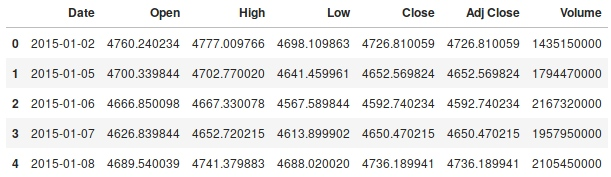
\includegraphics[width=\textwidth]{nasdaqTable}
	\caption{Sample of market data (NASDAQ)}
	\centering
\end{figure}

\section{Visualization}
It is vital to have the values correctly distributed. Market is unbalanced and the prices can range from 0 to infinity. For training it is best when the dataset has normal distribution (\cite{Distribution}), the histograms below do show that some kind of normalization will be needed.
EURUSD overall looks closer to what we need, but it is possible to get it better than that using normalization techniques.
Market data actually is normally distributed but only on short samples and only if there is no strong trend in the sample (in this case distribution looks like NASDAQ histograms).
\begin{figure}[h]
	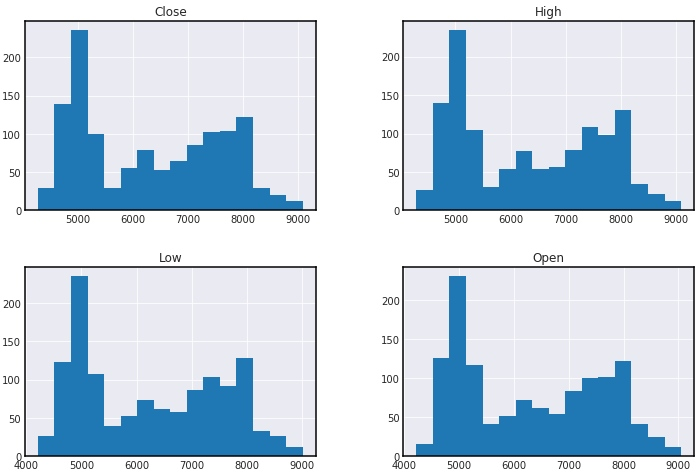
\includegraphics[width=\textwidth]{nasdaqHist}
	\caption{Histograms (NASDAQ)}
	\centering
\end{figure}
\begin{figure}[h]
	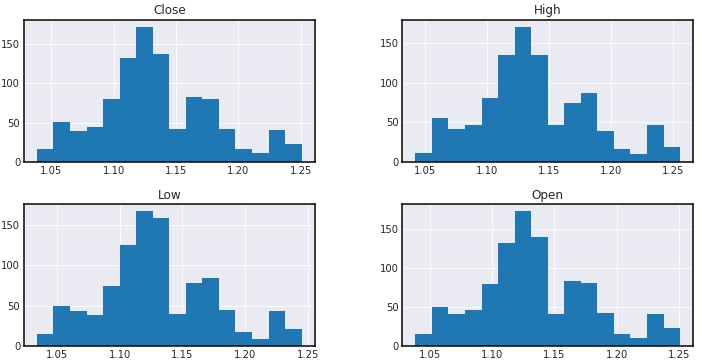
\includegraphics[width=\textwidth]{eurusdHist}
	\caption{Histograms (EURUSD)}
	\centering
\end{figure}

\section{Algorithms \& Techniques}

\section{Benchmark Model}

%%%%%%%%%%%%%%%%%%%%%%%%%

\part{Methodology}
\section{Data Preprocessing}
Knowing only the previous Open, High, Low and Close prices, we can produce some new features:
\begin{itemize}
	\item Gap -- days between entries, market is shut down for holidays resulting in gaps in the data.
	\item EMA -- exponential moving average.
	\item SMA -- simple moving average.
	\item Momentum -- value change indicator.
	\item RSI -- relative strength index oscillator.
\end{itemize}

\begin{figure}[h]
	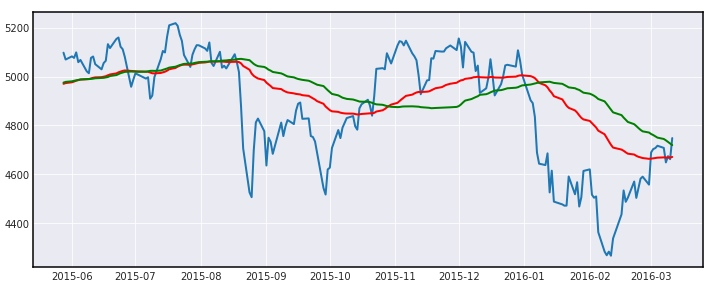
\includegraphics[width=\textwidth]{nasdaqClose}
	\caption{Close price (blue) with EMA (red) and SMA (green) indicators (NASDAQ)}
	\centering
\end{figure}
\begin{figure}[h]
	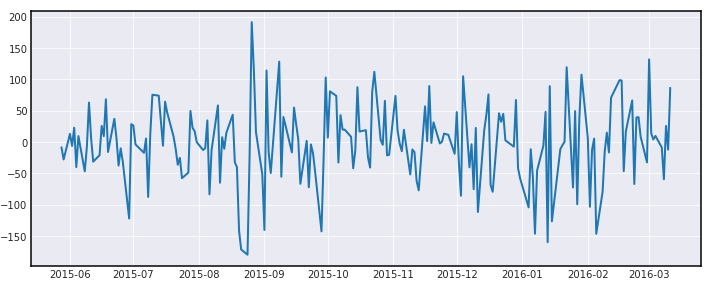
\includegraphics[width=\textwidth]{nasdaqMom}
	\caption{Momentum (NASDAQ)}
	\centering
\end{figure}
\begin{figure}[h]
	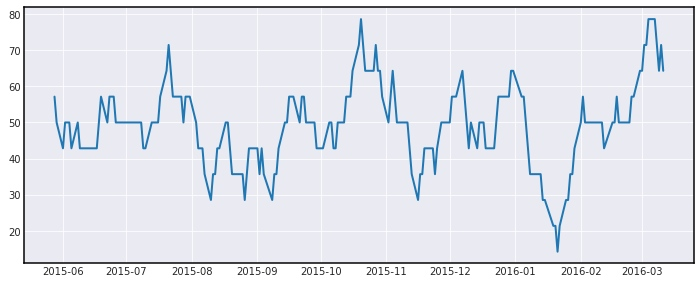
\includegraphics[width=\textwidth]{nasdaqRSI}
	\caption{Relative Strength Index (NASDAQ)}
	\centering
\end{figure}

\section{Implementation}
\section{Refinement}

%%%%%%%%%%%%%%%%%%%%%%%%%

\part{Results}
\section{Model Evaluation and Validation}
\section{Justification}

%%%%%%%%%%%%%%%%%%%%%%%%%

\part{Conclusion}
\section{Reflection}
\section{Further Improvements}

%%%%%%%%%%%%%%%%%%%%%%%%%

\pagebreak
\begin{thebibliography}{15}
	
\bibitem{Vidhya}
Aishwarya Singh, \textit{Stock Prices Prediction Using ML and DL Techniques},
\texttt{\href{https://www.analyticsvidhya.com/blog/2018/10/predicting-stock-price-machine-learningnd-deep-learning-techniques-python/}{analyticsvidhya.com}}

\bibitem{TowardsData}
Yibin Ng, \textit{Machine Learning Techniques applied to Stock Price Prediction}, \texttt{\href{https://towardsdatascience.com/machine-learning-techniques-applied-to-stock-price-prediction-6c1994da8001}{towardsdatascience.com}}

\bibitem{Distribution}
Rohit Sharma, \textit{Gaussian distribution}, \texttt{\href{https://medium.com/ai-techsystems/gaussian-distribution-why-is-it-important-in-data-science-and-machine-learning-9adbe0e5f8ac}{medium.com}}

%\bibitem{Khan}
%\texttt{\href{https://www.khanacademy.org/economics-finance-domain/core-finance/stock-and-bonds}{khanacademy.com}}

%\bibitem{Oscillators}
%\texttt{\href{https://www.fxcm.com/uk/insights/learn-forex-oscillators-and-momentum-indicators/}{fxcm.com}}

\bibitem{Yahoo}
Yahoo! Finance
\texttt{\href{https://finance.yahoo.com}{finance.yahoo.com}}

\bibitem{HistData}
HistData
\texttt{\href{http://histdata.com}{histdata.com}}

\end{thebibliography}

\end{document}


























